\documentclass{article}

\usepackage{amsmath}
\usepackage{multicol}
\usepackage{tikz}
\usetikzlibrary{automata, positioning}

\title{FULL SAT}
\author{Raudel Alejandro Gómez Molina}

\begin{document}

\maketitle

\section{Lenguaje FULL-SAT}

En esta sección se presentará un nuevo enfoque distinto a los anteriores, el cual se basa en definir un lenguaje al cual
pertenecen todos los problemas SAT que son satisfacible y al cual se le denominará \textit{FULL-SAT}.

\section{Transformación de una fórmula booleana a una cadena}

Primeramente para definir FULL-SAT se debe definir una transformación de una fórmula booleana a una cadena de símbolos.

Dada una fórmula booleana en CNF:
$$F=X_1 \wedge X_2 \wedge \ldots \wedge X_n$$
donde cada cláusula $X_i$ es una disyunción de literales:
$$X_i=L_{i1} \vee L_{i2} \vee \ldots \vee L_{im}$$
y cada literal $L_{ij}$ es una variable booleana o su negación. En cada cláusula $X_i$ las variables que aparecen en $F$,
puede tener cada una 3 estados posibles: $a$ si la variable aparece positiva, $b$ si la variable aparece negada y $c$ si la variable
no pertenece a ninguno de los literales de la cláusula.

Ahora dada la afirmación anterior, se puede definir una cadena de símbolos $w$
que representa a la cláusula $X_i$ sobre una secuencia de variables $v_1,v_2,\ldots,v_p$ de la siguiente manera:

\begin{itemize}
    \item $w$ cuenta con exactamente $p$ símbolos.
    \item Si la variable $v_j$ aparece positiva en $X_i$, entonces el $j$-ésimo símbolo es $a$.
    \item Si la variable $v_j$ aparece negada en $X_i$, entonces el $j$-ésimo símbolo es $b$.
    \item Si la variable $v_j$ no aparece en $X_i$, entonces el $j$-ésimo símbolo es $c$.
\end{itemize}
Si se toma la secuencia de variables correspondiente a $F$, y se le aplica el procedimiento anterior a cada cláusula
se obtendrá una cadena de símbolos que representa a dicha cláusula en $F$.

Si ya se tiene una representación para cada cláusula de $F$ solo resta obtener una cadena de símbolos que represente a $F$,
esto se puede lograr concatenando las cadenas de símbolos de cada cláusula de $F$ en el orden que aparecen con un separador
en este caso se eligió el símbolo $d$.

Por ejemplo la siguiente fórmula booleana en \textit{CNF}:
$$F=(x_1 \vee x_2) \wedge (\neg x_1 \vee x_2 \vee x_3) \wedge (x_1 \vee \neg x_2 \vee x_3)$$
puede ser expresada como la cadena de símbolos:
$$w=aacdbaadabad$$
tomando como secuencia de variables $x_1, x_2, x_3$ como se describió anteriormente.

\subsection{Definición del lenguaje FULL-SAT}

El lenguaje FULL-SAT se define como $L_{FULL_SAT}=\{w\,|\,w \in L_{CNF} \wedge f_{SAT}(w)\}$, donde $L_{CNF}$ representa el lenguaje
de todas las fórmulas booleanas en CNF y $f_{SAT}(w)$ es una función que determinista si $w$ es satisfacible.

En las próximas secciones se presentarán varios enfoques para definir $f_{SAT}$.

\section{Transductor FULL-SAT}

En esta sección la idea para definir $f_{SAT}$ es construir un transductor finito que acepte como entrada cadenas del lenguaje $L_{0,1}=\{wd\}^+$ donde $w\in \{0,1\}^*$
y tenga como salida cadenas, donde cada cadena $e$ representa una fórmula booleana en \textit{CNF} y que acepte si y solo si la fórmula es satisfacible. Detrás
de esta construcción se busca asociar cada carácter 0 ó 1 en la cadena de entrada al valor de la variable booleana correspondiente en la cadena de salida y verificar que para dichos
valores al evaluar la fórmula booleana se obtenga un valor de verdad. Observe que mediante esta construcción se mantiene la invariante fundamental del SAT que a dos instancias
de la misma variable se les asocia el mismo valor de verdad, esto es posible por como está definido el formato de la cadena de entrada.

A continuación se define el transductor finito $T_{SAT}$ que sigue la construcción definida anteriormente, para ello se define
el transductor $T_{CLAUSE}$ (Figura \ref{fig:transducer}) que hace el proceso de transducción para los valores de verdad de una cláusula $w$, donde $w\in \{0,1\}$:

\[
    T_{CLAUSE} = (Q, {\Sigma}, \Gamma, \delta, q_{0}, F),
\]
donde:
\begin{itemize}
    \item \(Q\) = ${q_0,q_p,q_n}$.
    \item \(\Sigma\) = ${0,1}$.
    \item \(\Gamma\) = ${a,b,c}$.
    \item \(\delta: Q \times \Sigma \to Q \times \Gamma^*\) función de transición.
    \item \(q_{0} = q_0\) estado inicial.
    \item \(F={q_p}\) conjunto de estados finales.
\end{itemize}
se define la función de transición $\delta$ de la siguiente manera:

\begin{itemize}
    \item  transiciones para el estado $q_0$: representa el estado inicial.
          \begin{multicols}{2}
              \begin{itemize}
                  \item $\delta_{SAT}(q_0,1)=(q_p,a)$
                  \item $\delta_{SAT}(q_0,0)=(q_n,a)$
                  \item $\delta_{SAT}(q_0,1)=(q_n,b)$
                  \item $\delta_{SAT}(q_0,0)=(q_p,b)$
                  \item $\delta_{SAT}(q_0,1)=(q_0,c)$
                  \item $\delta_{SAT}(q_0,0)=(q_0,c)$
              \end{itemize}
          \end{multicols}
          
    \item  transiciones para el estado $q_p$ (estado positivo de $T_{CLAUSE}$): representa que para los valores de verdad de la cláusula obtiene un valor de verdad positivo.
          \begin{multicols}{2}
              \begin{itemize}
                  \item $\delta_{SAT}(q_{p},1)=(q_{p},a)$
                  \item $\delta_{SAT}(q_{p},0)=(q_{p},a)$
                  \item $\delta_{SAT}(q_{p},1)=(q_{p},b)$
                  \item $\delta_{SAT}(q_{p},0)=(q_{p},b)$
                  \item $\delta_{SAT}(q_{p},1)=(q_{p},c)$
                  \item $\delta_{SAT}(q_{p},0)=(q_{p},c)$
              \end{itemize}
          \end{multicols}
          
    \item  transiciones para el estado $q_n$ (estado negativo de $T_{CLAUSE}$): representa que para los valores de verdad la cláusula obtiene un valor de verdad negativo.
          \begin{multicols}{2}
              \begin{itemize}
                  \item $\delta_{SAT}(q_{n},1)=(q_{p},a)$
                  \item $\delta_{SAT}(q_{n},0)=(q_{n},a)$
                  \item $\delta_{SAT}(q_{n},1)=(q_{n},b)$
                  \item $\delta_{SAT}(q_{n},0)=(q_{p},b)$
                  \item $\delta_{SAT}(q_{n},1)=(q_{n},c)$
                  \item $\delta_{SAT}(q_{n},0)=(q_{n},c)$
              \end{itemize}
          \end{multicols}
\end{itemize}

\begin{figure}[h]
    \centering 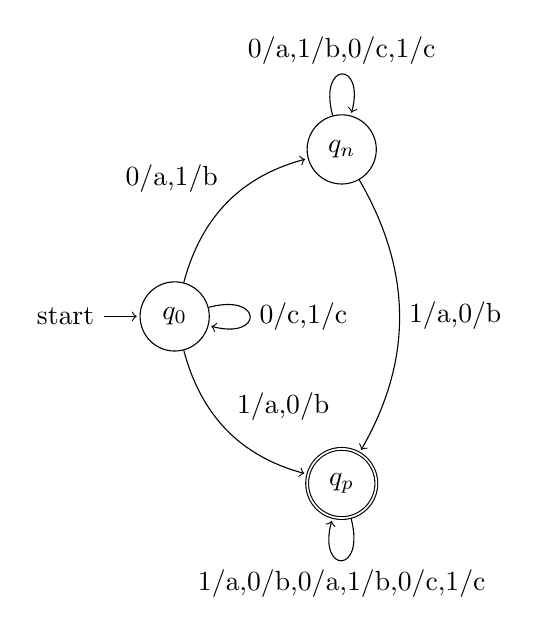
\begin{tikzpicture}[shorten >=1pt, node distance=3cm, on grid, auto]
        
        % Nodos
        \node[state, initial] (q0)   {$q_0$};
        \node[state] (qn) [above right=of q0] {$q_n$};
        \node[state, accepting] (qp) [below right=of q0] {$q_p$};
        
        % Transiciones
        \path[->]
        (q0) edge [bend left] node {0/a,1/b} (qn)
        (q0) edge [bend right] node {1/a,0/b} (qp)
        (q0) edge [loop right] node {0/c,1/c} (q0)
        
        (qn) edge [bend left] node {1/a,0/b} (qp)
        (qn) edge [loop above] node {0/a,1/b,0/c,1/c} (qn)
        
        (qp) edge [loop below] node {1/a,0/b,0/a,1/b,0/c,1/c} (qp);
        
    \end{tikzpicture}
    \caption{Transductor $T_{CLAUSE}$.}
    \label{fig:transducer} % Esto es para referenciar la figura en el texto
\end{figure}

Ahora para definir el transductor $T_{SAT}$ se toman dos instancias del transductor $T_{CLAUSE}$ ($T_1$ y $T_2$ respectivamente) y se concatenan
añadiendo una transición del estado $q_{p_1}$ (estado positivo de $T_1$) al estado $q_{0_2}$ (estado inicial de $T_2$) con el símbolo $d$ (tanto de
lectura como de escritura) y además se lenguaje agrega una clausura a $T_2$ con una transición del estado $q_{p_2}$
(estado positivo de $T_2$) al estado $q_{0_2}$ con el símbolo $d$ (tanto de lectura como de escritura). Entonces solo resta definir
el estado inicial y el estado final de $T_{SAT}$, los cuales serían $q_{0_1}$ (estado inicial de $T_1$) y $q_{0_2}$ (estado inicial de $T_2$),
respectivamente.

\subsection{Definición del lenguaje FULL-SAT usando transducción finita}

Finalmente se define el lenguaje FULL-SAT como el lenguaje de todas las cadenas $e$ que son aceptadas por el transductor $T_{SAT}$, a partir del lenguaje
de cadenas de entrada $L_{0,1}=\{wd\}^+$ donde $w\in \{0,1\}^*$. 

$$L_{FULL-SAT} = \{e\,|\,\exists w \in L_{0,1} \wedge e \in T_{SAT}(w) \}$$

Luego $L_{FULL-SAT}$ contiene todas las fórmulas booleanas satisfacibles, pero este conjunto por si solo no sirve de mucho sin un formalismo
que permita conocer si una cadena que representa una fórmula booleana pertenece al lenguaje o no, para ello se necesita encontrar un formalismo que sea capaz
de generar el lenguaje $L_{0,1}$ y al aplicarle el transductor $T_{SAT}$ a dicho formalismo se obtenga un formalismo que cuente con un algoritmo de parsing
para reconocer si una cadena pertenece a dicho formalismo o no.

Como se evidenció en esta sección encontrar un formalismo que genere el lenguaje $L_{0,1}$, el cual sea cerrado bajo transducción finita
es suficiente para generar el lenguaje $L_{FULL-SAT}$. Una pregunta interesante sería saber si la existencia de dicho formalismo
es una condición necesaria para definir el lenguaje $L_{FULL-SAT}$ otra pregunta interesante sería saber si existe un formalismo
que sea capaz de describir el lenguaje $L_{FULL-SAT}$ y el problema de la palabra en dicho formalismo sea polinomial (observe que de esta manera
se estaría resolviendo el problema \textbf{P vs NP}).

\section{FULL-SAT como lenguaje de índice global}

En esta sección se presentará una una forma de generar el lenguaje $L_{0,1}$ empleando una GIG. En \cite{globalIndexLanguages} se presenta
una GIG, $G_{ww^+}$ que genera el lenguaje $L(G_{ww^*})=\{ww^+\,|\,w\in\{a,b\}\}$: 
$$
    G_{ww^+} = (N, \Sigma, I, S, \#, P) 
$$
donde:

\begin{itemize}
    \item $N= \{S,R,A,B,C\}$.
    \item \( \Sigma=\{a,b\} \) .
    \item $I=\{i,j\}$.
    \item $S$ es el \textbf{símbolo inicial}.
    \item $\#$ es el \textbf{símbolo inicial de la pila}.
    \item $P$ es un conjunto finito de \textbf{producciones}:
          \begin{multicols}{2}
              \begin{itemize}
                  \item $S\underset{\varepsilon}{\to} AS\,|\,BS\,|\,C$
                  \item $C\underset{\varepsilon}{\to} RC\,|\,L$
                  \item $R\underset{\overline{i}}{\to} RA$
                  \item $R\underset{\overline{j}}{\to} RB$
                  \item $R\underset{[\#]}{\to} \varepsilon$
                  \item $A\underset{i}{\to} a$
                  \item $B\underset{j}{\to} b$
                  \item $L\underset{\overline{i}}{\to} La\,|\,a$
                  \item $L\underset{\overline{j}}{\to} Lb\,|\,b$
              \end{itemize}
          \end{multicols}
\end{itemize}

Observe que la pila en esta gramática es un mecanismo de memoria suficiente para generar el lenguaje \textit{Copy} como se
define en \cite{globalIndexLanguages}, a cada caracter de $\Sigma$ le corresponde un no terminal y un símbolo de la pila 
por el que se puede producir dicho caracter almacenando el caracter el símbolo de la pila correspondiente, el funcionamiento 
de la gramática lo compone además un mecanismo de recursión por el que se puede producir un no terminal asociado a un caracter
solo eliminando el símbolo de la pila asociado a dicho caracter por último el mecanismo de recursión produce la cadena vacía
solo si el símbolo inicial de la pila se encuentra en el tope.

Entonces dada esta gramática es relativamente realizar una modificación para generar el lenguaje $L_{0,1}$,
a esta nueva gramática se denominará $G_{0,1}$. Luego $G_{0,1}$ se define como:

$$
    G_{0,1} = (N, \Sigma, I, S, \#, P) 
$$
donde:

\begin{itemize}
    \item $N= \{S,R,A,B,C,D\}$.
    \item \( \Sigma=\{0,1,d\} \) .
    \item $I=\{i,j,k\}$.
    \item $S$ es el \textbf{símbolo inicial}.
    \item $\#$ es el \textbf{símbolo inicial de la pila}.
    \item $P$ es un conjunto finito de \textbf{producciones}:
          \begin{multicols}{2}
              \begin{itemize}
                  \item $S\underset{\varepsilon}{\to} AS\,|\,BS\,|\,DC$
                  \item $C\underset{\varepsilon}{\to} RC\,|\,L$
                  \item $R\underset{\overline{i}}{\to} RA$
                  \item $R\underset{\overline{j}}{\to} RB$
                  \item $R\underset{\overline{k}}{\to} RD$
                        
                  \item $R\underset{[\#]}{\to} \varepsilon$
                  \item $A\underset{i}{\to} a$
                  \item $B\underset{j}{\to} b$
                  \item $D\underset{k}{\to} d$
                  \item $L\underset{\overline{i}}{\to} L$
                  \item $L\underset{\overline{j}}{\to} L$
                  \item $L\underset{\overline{k}}{\to} L$
                  \item $L\underset{[\#]}{\to} \varepsilon$
              \end{itemize}
          \end{multicols}
\end{itemize}

Como modificaciones a la gramática anterior se ha introducido un nuevo terminal, un no terminal y un símbolo de la pila 
manteniendo la invariante de correspondencia que se mencionó anteriormente entre los elementos de estos 3 conjuntos. Por
otro se modificaron las producciones del no terminal $L$ para que unicamente produzca la cadena vacía eliminando todos Los
elementos de la pila, con ello se puede generar el lenguaje $L_{0,1}$.
\section{FULL-SAT como lenguaje de concatenación de rango}

En esta sección se presentará un enfoque para generar el lenguaje $L_{0,1}$ primeramente y luego para generar el lenguaje $L_{FULL-SAT}$.
Ambos enfoques usando gramáticas de concatenación de rango.

\subsection{$L_{0,1}$ como lenguaje de concatenación de rango}

Se define la gramática $G_{0,1}$ como sigue:
\[
    G_{0,1} = (N, T, V, P, S),
\]
donde:

\begin{itemize}
    \item $N=\{S,A,B,C,Eq\}$
    \item $=\{0,1,d\}$.
    \item $V=\{X,Y,P\}$.
    \item El conjunto de cláusulas $P$ es el siguiente:
          \begin{itemize}
              \item  $S(X)\to A(X)$
              \item $A(YdX)\to B(X,Y)C(X)$
              \item $B(XdY,P)\to B(Y,P) C(X) Eq(X,P)$
              \item $B(\varepsilon,Y)\to \varepsilon$
              \item $C(0X)\to C(X)$
              \item $C(1X)\to C(X)$
              \item $C(\varepsilon)\to \varepsilon$
          \end{itemize}
    \item El \textbf{símbolo inicial} es $S$.
\end{itemize}

El predicado $Eq$ se define en \cite{mainRCGBib} y comprueba que dos cadenas sobre un alfabeto sean iguales, por otro lado 
le predicado $B$ se encarga de definir la sustitución en rango de la próxima cadena de 0 y 1 y comprobar que este sea igual
al patrón inicial. De esta manera se pueden reconocer cadenas que pertenezcan al lenguaje $L_{0,1}$.

Como se mencionó anteriormente las RCG no son cerradas bajo transducción finita, por tanto no se puede realizar el mismo 
análisis que en las 2 secciones anteriores, esto no necesariamente impide que el lenguaje generado por la transducción finita del lenguaje que 
representa la gramática anterior no pueda cumplir ciertas características que permitan generar lenguaje $L_{FULL-SAT}$. 

\subsection{Otro enfoque para generar el lenguaje FULL-SAT}

A continuación se presentará una estrategia distinta para generar el lenguaje $L_{FULL-SAT}$, que no emplea el transductor $T_{SAT}$,
en este caso la función $f_{SAT}$ se define dentro del funcionamiento de la gramática para ello se define la siguiente RCG:
\[
    G_{FULL-SAT} = (N, T, V, P, S),
\]
donde:

\begin{itemize}
    \item $N=\{S,A,B,C,P,N,Cp,Cn\}$
    \item $=\{a,b,c,d\}$.
    \item $V=\{X,Y\}$.
    \item El \textbf{símbolo inicial} es $S$.
\end{itemize}

A continuación se desglosa el conjunto de \textbf{cláusulas} $P$ en varias fases agrupando las cláusulas
por funcionalidad:

\begin{itemize}
    \item $S(X)\to A(X)$
    \item \textbf{Primera fase:} El siguiente conjunto de cláusulas genera la cadena de 0 y 1 que que da valores a las variables de la
          fórmula booleana:
          \begin{multicols}{2}
              \begin{itemize}
                  \item $A(aX)\to P(X,1)$
                  \item $A(aX)\to N(X,0)$
                  \item $A(bX)\to N(X,1)$
                  \item $A(bX)\to P(X,0)$
                  \item $A(cX)\to N(X,1)$
                  \item $A(cX)\to N(X,0)$
                        
                  \item $P(aX,Y)\to P(X,Y1)$
                  \item $P(aX,Y)\to P(X,Y0)$
                  \item $P(bX,Y)\to P(X,Y1)$
                  \item $P(bX,Y)\to P(X,Y0)$
                  \item $P(cX,Y)\to P(X,Y1)$
                  \item $P(cX,Y)\to P(X,Y0)$
                  \item $P(dX,Y)\to B(X,Y)$
                        
                  \item $N(aX,Y)\to P(X,Y1)$
                  \item $N(aX,Y)\to N(X,Y0)$
                  \item $N(bX,Y)\to N(X,Y1)$
                  \item $N(bX,Y)\to P(X,Y0)$
                  \item $N(cX,Y)\to N(X,Y1)$
                  \item $N(cX,Y)\to N(X,Y0)$
              \end{itemize}
          \end{multicols}
          
          El predicado $A$ representa el primer predicado reconocimiento de este se deriva a los predicados $P$
          (representa que la cláusula de la fórmula booleana se encuentra en un estado de verdad positivo) 
          y $N$ (representa que la cláusula de la fórmula booleana se encuentra en un estado de verdad negativo)
          en dependencia del valor de la instancia de la variable correspondiente. El predicado $P$ deriva hacia
          sí mismo independientemente del símbolo, exceptuando el símbolo $d$, caso en el que se procede a la siguiente
          fase.
          El funcionamiento de esta face es prácticamente el mismo de descrito en el transductor $T_{SAT}$.
          
    \item \textbf{Segunda fase:} El siguiente conjunto de cláusulas se encarga de un mecanismo de clausura que le permite a la gramática
          reconocer si la asignación realiza en la fase anterior es válida para las restantes cláusulas de la fórmula
          booleana.
          \begin{itemize}
              \item $B(X_1dX_2,Y)\to C(X_1,Y) B(X_2,Y)$
              \item $B(\varepsilon,Y)\to\varepsilon$
          \end{itemize}
          
          El predicado $B$ permite realizar la clausura mientras que le predicado $C$ comprueba que la cláusula de la fórmula
          booleana actual sea satisfacible.
          
    \item \textbf{Tercera fase:} Solo resta definir el comportamiento de $C$:
          \begin{itemize}
              \begin{multicols}{2}
                  \item $C(X,Y)\to Cn(X,Y)$
                  
                  \item $Cn(aX,1Y) \to Cp(X,Y)$
                  \item $Cn(aX,0Y) \to Cn(X,Y)$
                  \item $Cn(bX,1Y) \to Cn(X,Y)$
                  \item $Cn(bX,0Y) \to Cp(X,Y)$
                  \item $Cn(cX,1Y) \to Cn(X,Y)$
                  \item $Cn(cX,0Y) \to Cn(X,Y)$
                  
                  \item $Cp(aX,1Y) \to Cp(X,Y)$
                  \item $Cp(aX,0Y) \to Cp(X,Y)$
                  \item $Cp(bX,1Y) \to Cp(X,Y)$
                  \item $Cp(bX,0Y) \to Cp(X,Y)$
                  \item $Cp(cX,1Y) \to Cp(X,Y)$
                  \item $Cp(cX,0Y) \to Cp(X,Y)$
                  \item $Cp(\varepsilon,\varepsilon)\to \varepsilon$
              \end{multicols}
          \end{itemize}
          
          Observe que este funcionamiento es exactamente igual al de la primera fase con un predicado que representa un estado
          positivo ($Cp$) y un predicado que representa un estado
          positivo ($Cn$) pero esta vez no se genera la cadena sino que se comprueba con un patrón predefinido en la primera
          fase.
          
          Ahora como $G_{FULL-SAT}$ reconoce las fórmulas booleanas satisfacibles solo se debe analizar el problema de la
          palabra para determinar si una fórmula es satisfacible.
          
          \subsubsection{Análisis de la complejidad computacional}
          
          Como se mencionó anteriormente no todas las RCG tienen un algoritmo de parsing lineal y $G_{FULL-SAT}$ es un ejemplo de 
          ello, observe que en la primera fase se genera la cadena binaria que representa la asignación de valores a las variables
          booleanas y dicha cadena participa en los predicados de fases posteriores. Si se analiza el algoritmo de parsing descrito en 
          \cite{mainRCGBib} un factor en la complejidad del algoritmo de parsing es la cantidad de rangos posibles para una cadena 
          que debe ser reconocida por un predicado y en este caso la cadena que estamos analizando puede tomar $2^n$ valores distintos, donde
          $n$ es la cantidad de variables en la fórmula booleana por lo que la cantidad de rangos sería $n^22^n$, pero esta es una cota
          burda ya que una vez generada la cadena de asignación por la forma de la gramática solo se utiliza un solo rango que se va construyendo
          bajo demanda. El resto de las fases de la gramática tienen una complejidad de $m^2$ donde $m$ es la cantidad de caracteres
          en la cadena de entrada, por lo que la complejidad total sería $O(2^nm^2)$.
          
          Este es un resultado interesante ya que demuestra que no es necesario usar el transductor $T_{SAT}$ para definir el 
          lenguaje $L_{FULL-SAT}$, mediante formalismo de escritura regulada.
          
          
\end{itemize}

\bibliographystyle{plain}
\bibliography{../Bibliography}


\end{document}
